\documentclass[12pt,a4paper,twoside]{article}
\usepackage{amsmath}
\usepackage{physics}
\usepackage{amssymb}
\usepackage{graphicx}
\begin{document}

\subsection{Multiple importance sampling}

Monte-Carlo sampling is a simple and convenient technique to integrate a function over a specific domain. The only thing required is to know the distribution from which samples are drawn and to be able to draw samples from this domain. The expected value of Monte-Carlo sampling will in the limit converge to the actual integral value of the function that is being integrated.

Monte-Carlo estimator is defined as:

\begin{equation}
\label{monte-carlo-estimator}
F_N = \frac{1}{N} \sum_{i=1}^N \frac{f(X_i)}{p(X_i)}
\end{equation}


Importance sampling is a variance reduction technique. The idea behind importance sampling is that the Monte-Carlo estimator converges more quickly when samples are taken from a distribution $p(x)$ that is similar to the function $f(x)$ in the integrand~\cite{pbrtv3}. This means samples that are affecting the result more, or are more important, are sampled with a higher probability.

To apply importance sampling, one needs to compute the probability density function $p(x)$ by integrating over the distribution to find a normalization factor to normalize the probability density function. Once the $p(x)$ is known you can randomly draw samples from the sample domain and use equation~\ref{monte-carlo-estimator} to find the result of the integral. 

There are different way to draw samples. If the distribution to sample from can easily be integrated and inverted, then inversion sampling is a good candidate. Another way is rejection sampling. In this thesis I will mainly use inversion sampling. When inversion sampling is not possible analytically, then I will use known tricks to sample from a given domain.

\subsubsection{Multiple importance sampling}

Usually when drawing samples from a complex material description, the material can be subdivided in the product of two functions $f(X)g(X)$. In this case it is likely that you can find a distribution that works great for reducing the variance for function $f(X)$. Averaging the result makes things worse, because averaging variance, you can come up with a distribution that samples efficiently for a specific situation, but does not work well in other circumstances. Multiple importance sampling lets you combine two or more sampling distributions efficiently to further reduce variance and to faster converge to the result.

\begin{align}
F_N = \frac{1}{n_f} \sum_{i=1}^{n_f} \frac{f(X_i) g(X_i) w_f(X_i)}{p_f(X_i)} + \frac{1}{n_g} \sum_{j=1}^{n_g} \frac{f(Y_j)g(Y_j)w_g(Y_j)}{p_g(Y_j)}
\end{align}

In this equation $n_f$ and $n_g$ are the amount of samples taken from sample distributions $p_f$ and $p_g$ respectively. We can not just average the terms, because variance is additive as in $Var(X+Y) = Var(X) + Var(Y)$. The weighting factor $w_s$ solves this problem by weighting the samples over the distribution. A weighting function that is usually taken is the balance heuristic.

\begin{align}
w_s(x) \frac{n_s p_s(x)}{\sum_i n_i p_i(x)}
\end{align}

This weighting function . If there is only one distribution to sample from, the weighting factor will always be 1. If there are multiple distributions to sample from it takes into account the number of samples taken from these distributions and their corresponding probability of being sampled.

PBRT already implements multiple importance sampling for lighting and materials. This means that the estimator function is already implemented in a so called integrator. In order to comply with PBRT, the dual scattering material should provide an implementation for the probability density function and for drawing samples from their respective distributions.



\subsection{Identifiying importance sampling functions for Dual Scattering Approximation}
When doing importance sampling, we like to sample an incident direction $\omega_i$ given an outgoing direction $\omega_o$. The idea is to put more emphasis on samples that are important to the rendering equation than on samples that have a small effect.

Finding importance sampling functions for the dual scattering approximation requires finding functions in the rendering equation from which we can easily create a sample function.
To sample, we must obtain a pdf that is similar in shape to the rendering equation. Then this pdf must be integrated to a CDF and consequently this CDF must be inversed to be able to sample a direction vector, given a canonical random variable $\xi \in [0, 1]$.

The dual scattering algorithm can be defined as:

\begin{align}
f(\omega_i, \omega_r) & = (F^{\textnormal{direct}} + F^{\textnormal{scatter}}) \cos \theta_i\\
F^{\textnormal{direct}} & = f_s^{\textnormal{direct}} + d_b f_{\textnormal{back}}\\
f^{\textnormal{direct}}_s & = M_RN_R(\theta, \phi) + M_{TT}N_{TT}(\theta, \phi) + M_{TRT}N_{TRT}(\theta,\phi)\\
f^{\textnormal{back}}_s & = 2A_b(\theta) \cdot g(\sigma_b^2 + \sigma_f^2, \theta_d + \theta_o -\Delta_b)\\
\\
F^{\textnormal{scatter}} & = T_f \cdot d_f \cdot (f^{\textnormal{scatter}}_s + \pi d_b f_{\textnormal{back}})\\
f^{\textnormal{scatter}}_s & = M^G_RN^G_R(\theta, \phi) + M^G_{TT}N^G_{TT}(\theta, \phi) + M^G_{TRT}N^G_{TRT}(\theta,\phi)\\
M^G_{X \in \{\textnormal{R, TT, TRT}\}} & = g(\beta_X^2 + \sigma_f^2, \theta - \alpha_X)\\
N^G_{X \in \{\textnormal{R, TT, TRT}\}} & = \frac{1}{\pi} \int_{-\frac{\pi}{2}}^{\frac{\pi}{2}} N_X(\theta, \phi') \dd{\phi'}
\end{align}

All these functions have the potential to be importance sampled. Some functions might be similar to sample from. It might even be possible that uniform sampling will in the end still give the best result.

\subsubsection{Importance sampling the longitudinal equations from Marschner $M_R$ equation}
\label{importance-sampling-marschner-R}

The longitudinal functions for the Marschner model $M_{\textnormal{R}}, M_{\textnormal{TT}}, M_\textnormal{{TRT}}$ are all Gaussian functions with a different mean (longitudinal shift $\alpha$) and standard deviation (longitudinal width $\beta$).

\begin{equation}
M_{X \in \{\textnormal{R, TT, TRT}\}} = g(\beta_X, \theta_h - \alpha_X)
\end{equation}

The gaussian function cannot be analytically integrated and inverted~\cite{pixarmemo}. To generate samples we need to resort to compute the inverse error function or numerical inversion~\cite{pixarmemo}. Another option is to make use of the Box-Muller tranform. The Box-Muller transform takes two uniformly distributed samples in the interval [0, 1] and maps them to two standard normally distributed samples~\cite{box-muller}.

\begin{eqnarray}
X = \sqrt{-2 \ln u_1} \cos 2\pi u_2 \\
Y = \sqrt{-2 \ln u_1} \sin 2\pi u_2 
\end{eqnarray}

The idea is to first sample from a gaussian distribution and then adjust the value to incorporate the effects of the width and shift of the scattering lobes. Since the Gaussian distribution can lead to samples outside the allowed range, we have to make sure to clamp $\theta_h$ values below a certain maximum $\theta_{max}$ that depends on $\theta_r$ and the shift of the lobe $\alpha_X$. The sampled incident longitudinal angle can now easily be computed as $\theta_i = 2\theta_h - \theta_r$.

\begin{align}
\theta_{\textnormal{max}} & = \frac{\pi}{2} - \left| \frac{\theta_r}{2} - \alpha_X\right| \\
\theta & = \beta_{X} \cdot \sqrt{-2 \ln u_1} \cos 2\pi u_2) & \textnormal{with $u_1, u_2 \in [0, 1]$}  \\
\theta_h & = \theta + \alpha_X & \textnormal{with $\left|\theta\right| \leq \theta_{\textnormal{max}}$}\\
\theta_i & = 2 \theta_h - \theta &&
\end{align}

Since we are using a normalized Gaussian distribution to sample from, the probability density function is known to be as follows.

\begin{equation}
p_{M_{X \in \{\textnormal{R, TT, TRT}\}}}(\theta) = \frac{1}{\beta_{X} \sqrt{2\pi}} \cdot e^{-\frac{1}{2}(\frac{\theta}{\beta_{X}})^2}
\end{equation}


\subsubsection*{Importance sampling the Marschner $N_{TT}$ equation}

The Marschner model consists of a seperation of longitudinal scatterig and azimuthal scattering. can be importance sampled using s simplification described in~\cite{sadeghi:10} 

\begin{equation}
N_{TT}(\phi) = g(\beta_{TT}, \pi - \phi)
\end{equation}


As described in section~\ref{importance-sampling-marschner-R} we can use the Box-Muller transform to sample from a Gaussian distribution. 
The generated samples $\phi$ are unbounded, meaning that they can be outside the range for $\phi \in [\-\pi, \pi]$. A way to solve this is to clamp the values to this range. Since this can lead to a bias in the sampling process, the likelihood of sampling outside of the range is very small and hardly noticable in the renderings~\cite{pixarmemo}.

\begin{align}
\phi & = \beta_{TT} \cdot \sqrt{-2 \ln u_1} \cos 2\pi u_2) & \textnormal{with $u_1, u_2 \in [0, 1]$}  \\
\phi_i & = \phi_r - (\pi - \phi) &&
\end{align}


Take into account that $\phi_i$ in itself must be wrapped properly to stay inside it's range as well.

Since we are sampling from a normalized gaussian function, we already have the pdf. Filling in the width $\beta_{TT}$ the pdf looks like.

\begin{equation}
p_{N_{TT}}(\phi) = \frac{1}{\beta_{TT} \sqrt{2\pi}} \cdot e^{-\frac{1}{2}(\frac{\phi}{\beta_{TT}})^2}
\end{equation}


\subsubsection*{Importance sampling the Marschner azimuthal equations $N_R$ and $N_{TRT}$ from Marschner}

The Marschner azimuthal angles can be simplified by depending only on $\phi$ angles~\cite{sadeghi:10}. This simplification helps enormously to find a sampling function from the distributions.

\begin{align}
N_R = N_{TT} = \cos \frac{\phi}{2}
\end{align}

To sample from this distribution, we must perform some standard integrations to find the normalized probability density function. Then we can integrate the pdf to end up with a cumulative distribution function and subsequently inverse the function to have the inverse CDF to be able to sample from.

To find a probability density function $p(\phi)$ we must find a normalization factor $c$ such that the integral for $N_{R, TRT}$ from $\phi \in [-\pi, \pi]$ integrates to one. This derivation process is rather straightforward.

\begin{equation}
\int_{-\pi}^{\pi} p(\phi) \dd{\phi} = c \cdot \int_{-\pi}^{\pi} \cos \frac{\phi}{2} \dd{\phi} = 1
\end{equation}

To find the normalization factor we integrate over $\phi$.

\begin{align}
\frac{1}{c} & = \int_{-\pi}^{\pi} \cos \frac{\phi}{2} \dd{\phi} \\
 & = 2 \cdot \int_{-\frac{\pi}{2}}^\frac{\pi}{2} \cos u \dd{u}  & \textnormal{where  $u = \frac{\phi}{2}$}\\
 & = 2 \cdot \left[ \sin \frac{\phi}{2} \right]_{-\pi}^{\pi} = 2 \cdot (\sin \frac{\pi}{2} - \sin \frac{-\pi}{2}) = 4
\end{align}

The resulting normalization factor is $c = \frac{1}{4}$ which is used to normalize the probability density function. The cumulative distribution function $P$ follows similarly from the integral derivation we have just performed.

\begin{equation}
p(\phi) = \frac{ \cos \frac{\phi}{2}}{4} \cdot
\end{equation}

 \begin{align*}
P(\phi) & = \int_{-\pi}^{\phi} p(\phi') \dd{\phi'} = \int_{-\pi}^{\phi} \cos \frac{\phi'}{2} \dd{\phi'} \\
&  = 2 \cdot \left[\sin \frac{\phi'}{2} \right]_{-\pi}^{\phi} = 2 \cdot \left(\sin \frac{\phi}{2} + 1\right) \\
\end{align*}

The CDF maps the sample to the cumulative distribution probability, which starts at 0 and goes to 1. What we need is the inverse of the CDF to map from a cumulative probability value to a sample value. To be able to do this we need to invert the CDF to obtain the inverse cumulative distribution function. The inverse cumulative distribution function $P^{-1}(\xi)$ takes a canonical random uniform variable $\xi \in [0, 1]$, which maps back to a sample value $\phi$. Inversion is not so difficult and is show in equation~\ref{inverse_Nr}.

\begin{equation}
\phi = P^{-1}(\xi) = 2 \cdot \sin^{-1} \left( \frac{\xi}{2} - 1\right)
\end{equation}

\subsubsection*{Transmittance function}
\begin{equation}
T_f(n, \omega_i) = d_f \cdot \prod_{k=1}^{n} a_f(\theta_d) = d_f \cdot a_f(\theta_d)^n
\end{equation}
The transmittance function $T_f$ is not a pure material description that depends on incoming and outgoing directions. It also depends on the number of scatter events $n$ found along the incident lighting direction $\omega_i$. We do not know $\omega_i$, because this is the direction we are trying to sample in the first place.

In figure~\ref{fig:average_ab_af} the amount of average forward scattered light is displayed for different $\theta_d$. It is shown for nonabsorbing hair, blonde hair and brown hair for different scatter counts. As we expect, blonde hair transmits more energy through the fiber in the front hemisphere compared to brown hair. The difference between hair colors is primarily in the amount of absorbed light. It does not change the scattering behavior. As the number of scattering counts increases, the contribution of samples around $\theta_d = 0$ will become more significant, because of the power to $n$ in $a_f^n$. However, the contribution also fades away by the power of $n$.By taking into account the relevance around $\theta_d = 0$ I decided to base the shape on $cos \theta_d$. Taking into account that the integral sums to one, one ends up with the following probability density function $p$, cumulative distribution function and it's inverse.

\begin{align}
p_{a_f}(\theta_d) & = \frac{1}{2} \cos \theta_d \\
P_{a_f}(\theta_d) & = 1 + \sin \theta_d\\
P^{-1}_{a_f}(\xi) & = \theta_d = \sin^{-1}(\xi - 1) \\
\end{align}

\begin{figure}
  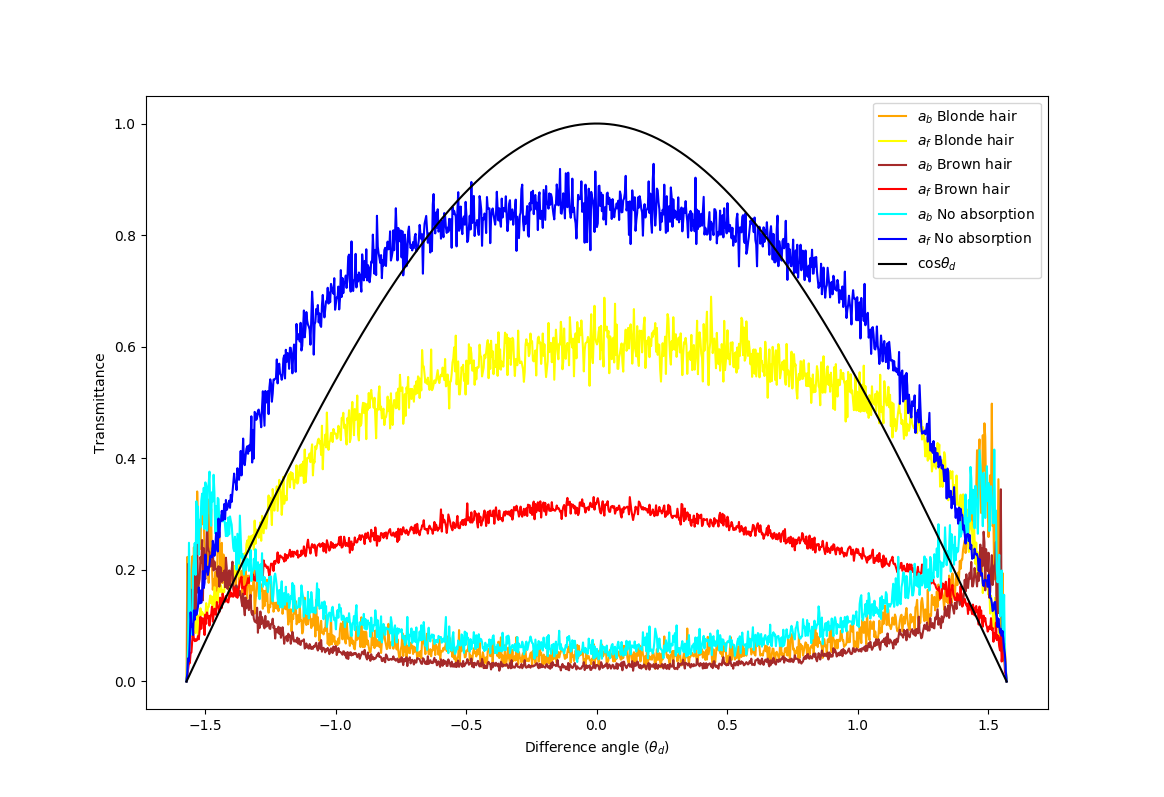
\includegraphics[width=\linewidth]{average_forward_backward_scattering_attenuation.png}
  \caption{Showing the average forward and backward transmittance. Nonabsorbing hair forward transmits a lot more light compared with colored hair. Also it can be seen that as the difference angle comes closer to +/-90 degrees, more light gets reflected back in the back hemisphere.}
  \label{fig:average_ab_af}
\end{figure}


\begin{align*}
M_X & = g(\beta_X^2, \theta_h - \alpha_X) \\
N_R & = \cos\frac{\phi}{2} \\
N_{TT} & = g(\gamma_{TT}^2, \pi - \phi) \\
N_{TRT} & = \cos\frac{\phi}{2} \\
M_R^G & = g
\end{align*}


\subsubsection*{Importance sampling for $N^G$}

\begin{equation}
\begin{split}
N_R^G(\theta) & = \frac{1}{\pi} \cdot \int_{-\frac{\pi}{2}}^{\frac{\pi}{2}} \cos \frac{\phi'}{2} \dd{\phi'} \\
 & = \frac{2}{\pi} \int \cos u \dd{u}  = \frac{2}{\pi} \cdot \sin u \\
 & = \frac{2}{\pi} \cdot \left[\sin \frac{\phi}{2}\right]_{-\frac{\pi}{2}}^{\frac{\pi}{2}} = \frac{4}{\pi}
\end{split}
\end{equation}

It turns out that $N_R^G$ is dependent only on $\phi$, but in such a matter that $\phi$ is only relevant for front scattered radiance. To sample a $\phi$ we can just uniformly sample from the front hemisphere, giving the following PDF.

\begin{equation}
p_{N^G_R}(\phi) = \frac{1}{\pi}
\end{equation}

More to follow...

\begin{figure}
  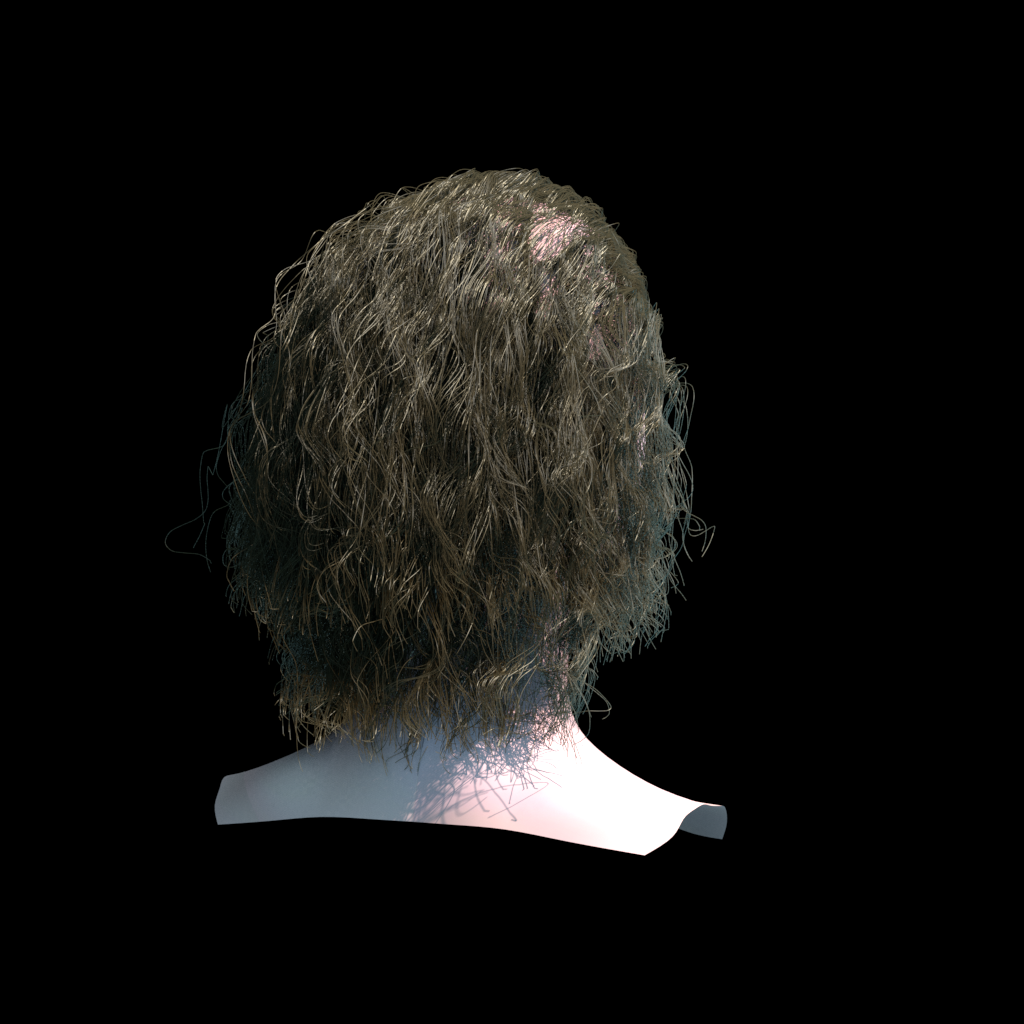
\includegraphics[width=\linewidth]{curly_blonde_dualscattering.png}
  \caption{Rendered using importance sampling for $M_R$ only.}
  \label{fig:dualscattering:blonde:MR}
\end{figure}



\bibliographystyle{ieeetr}
\bibliography{dualscattering_mis} 
\end{document}